%This work is licensed under the Creative Commons
%Attribution-ShareAlike 4.0 International License. To view a copy of
%this license, visit http://creativecommons.org/licenses/by-sa/4.0/ or
%send a letter to Creative Commons, PO Box 1866, Mountain View, CA
%94042, USA.

%\documentclass[gray,handout, pdftex, 11pt]{beamer}
%\documentclass[handout, pdftex, 11pt]{beamer}
\documentclass[pdftex, 11pt]{beamer}

\usepackage[utf8]{inputenc}
\usepackage[T1]{fontenc}
\usepackage{lmodern}
%\usepackage[italian]{babel}
\usepackage{graphicx}
\usepackage{microtype}
\usepackage{acronym}
\usepackage{array}
\definecolor{links}{HTML}{2A1B81}
\hypersetup{colorlinks,linkcolor=links,urlcolor=links}

\definecolor{links}{HTML}{2A1B81}
\hypersetup{colorlinks,linkcolor=,urlcolor=links}


\mode<presentation>{
  %-------------------------1
  \usetheme{Boadilla}
  \usecolortheme{beaver}
  %-------------------------1
  %-------------------------2
  %\usetheme{Goettingen}
  %\usecolortheme{sidebartab}
  %-------------------------2
  %\useoutertheme[right]{sidebar}
  %\usefonttheme{default}
  \setbeamercovered{transparent}
  %\setbeameroption{show notes on second screen=right}
  \setbeamertemplate{navigation symbols}{}
  \setbeamertemplate{footline}{}

  \bibliographystyle{abbrv}  
  %\renewcommand\bibfont{\scriptsize}
  \setbeamertemplate{bibliography item}{\textbullet}
  \setbeamertemplate{itemize item}{\checkmark}
  \setbeamertemplate{itemize subitem}{-}
  \setbeamertemplate{enumerate items}[default]
  \setbeamertemplate{sections/subsections in toc}[square]
}

\title[Lession 1]{\textbf{Logical Computational Thinking}}
\subtitle{Lession 1}
\institute[Tecnológico de Monterrey]{
  
\includegraphics[width=5cm]{img/logoTEC.jpg}
}

\author[Stefano Martina]{
  %\\[0.2cm]
  \textbf{Stefano MARTINA}\\
  {\small stefano.martina@gmail.com}
}

\date[3/9/15]{\flushright 3 September 2015}

\begin{document}

\begin{frame}[plain]
  \titlepage
  {\tiny \href{http://creativecommons.org/licenses/by-sa/4.0/}{
\includegraphics[width=1cm]{img/logoCC.png}} This work is licensed under a
    \href{http://creativecommons.org/licenses/by-sa/4.0/}{Creative
      Commons Attribution-ShareAlike 4.0 International License}.}
\end{frame}

\begin{frame}
  \frametitle{Material}
  \begin{block}{Material}
    all the material will be available at \url{https://github.com/trianam/courseLCT1516}
  \end{block}
  \pause
  \begin{block}{Book}
    \url{https://www.dropbox.com/s/umx65z3m9bnm6xj/Metodologia_de_la_programacion__3ra_Edicion_-_Osvaldo_Cairo_Battistutti.pdf}
  \end{block}
\end{frame}

\begin{frame}
  \frametitle{Evaluation}
    \begin{itemize}
  \item You will be evaluated continuously along the lectures
    \begin{itemize}
    \item exercises
    \item questions
    \item etc...
    \end{itemize}
  \item and with exams
    \begin{itemize}
    \item 2 partials
    \item 1 final (project)
    \end{itemize}
  \end{itemize}
\end{frame}

\begin{frame}
  \frametitle{History}
  \begin{itemize}
  \item classical age and middle ages: \alert{algorisms} \\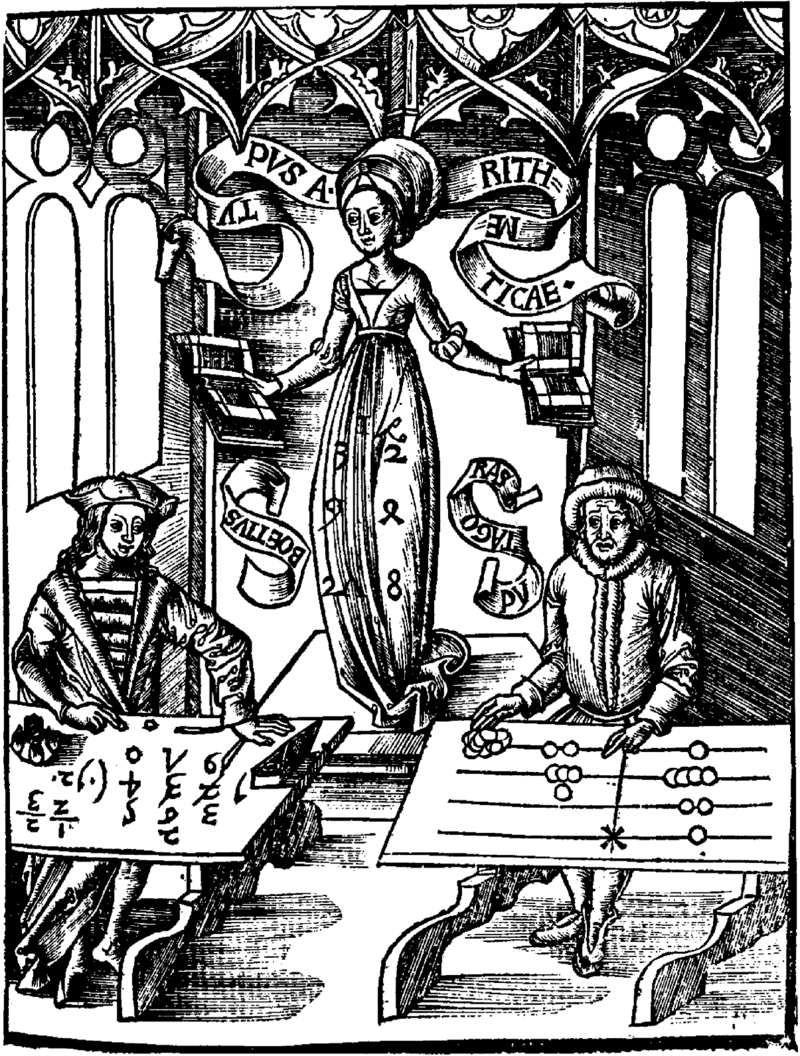
\includegraphics[width=2cm]{img/algorism.png}
  \item 1833-1842: \alert{Analytical engine} of Charles
    Babbage (Ada Byron) \\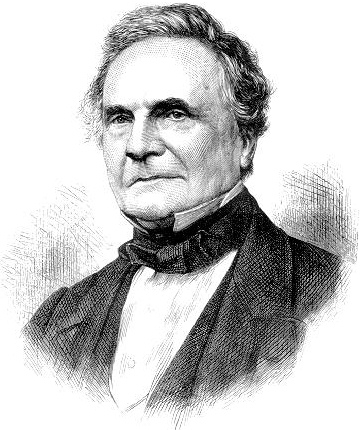
\includegraphics[width=2cm]{img/babbage.jpg}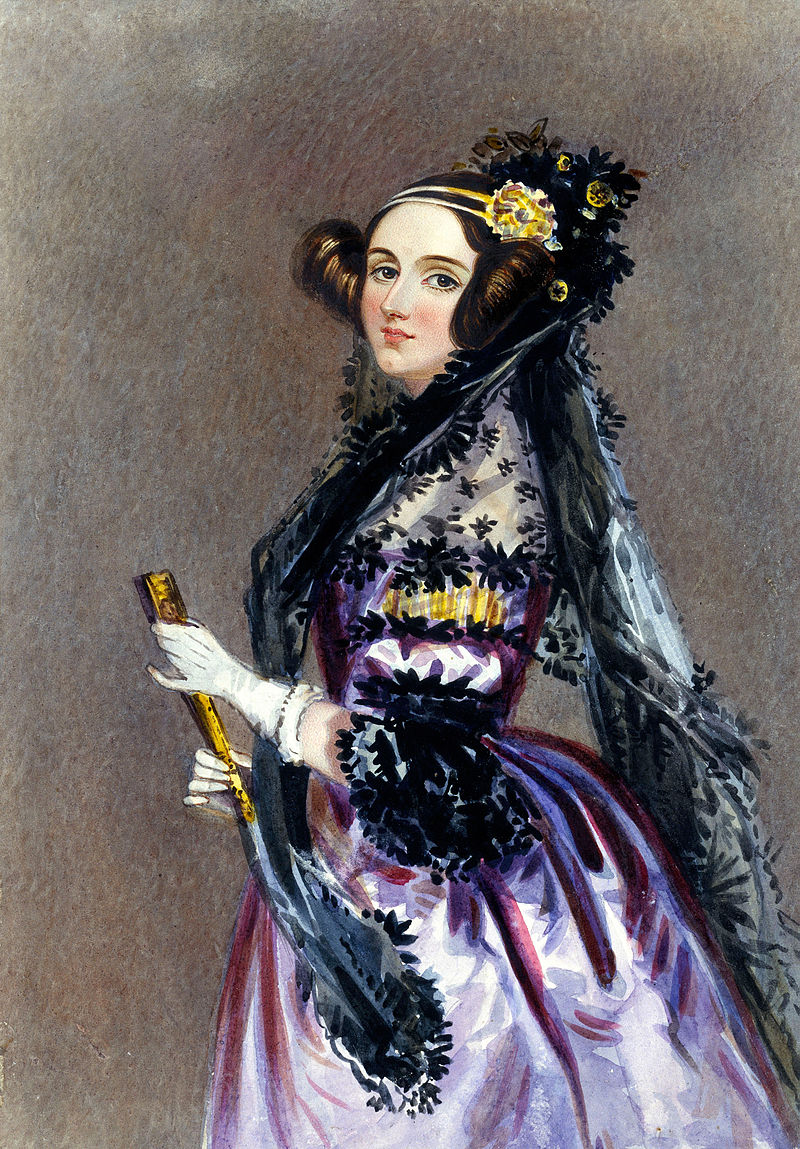
\includegraphics[width=2cm]{img/lovelace.jpg}
  \end{itemize}
\end{frame}

\begin{frame}
  \frametitle{History}
  \begin{itemize}
  \item before and during WW2: first modern computers (single purpose,
    programmable), \alert{Turing} studies \\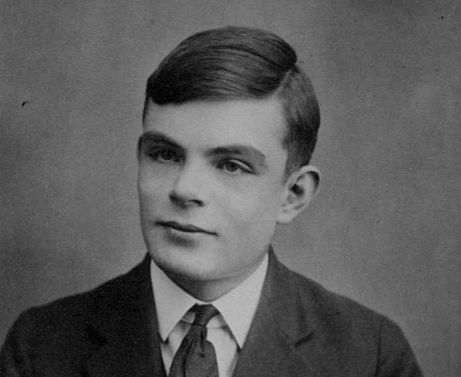
\includegraphics[width=2cm]{img/turing.jpg}
  \item 1946: \alert{ENIAC} (general purpose) \\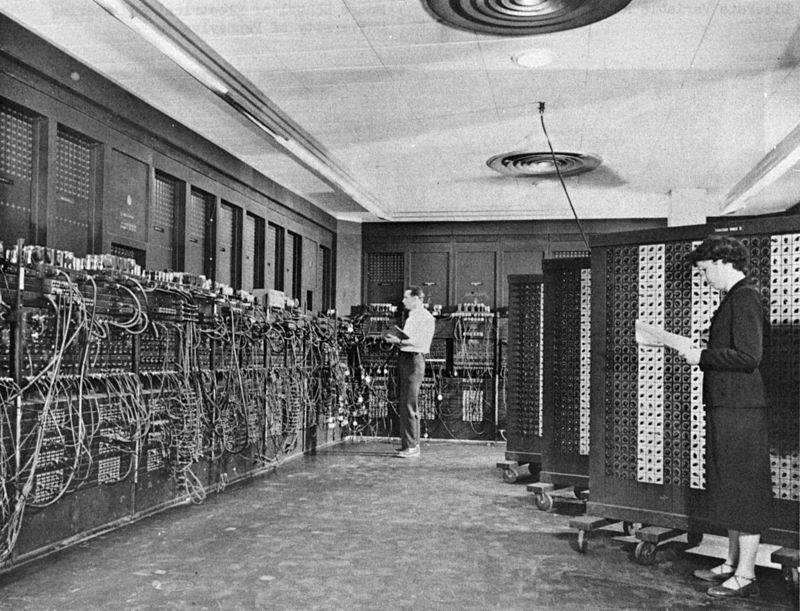
\includegraphics[width=2cm]{img/eniac.jpg}
  \item 1951: \alert{EDVAC}, Von Neumann architecture \\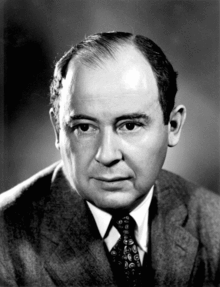
\includegraphics[width=2cm]{img/vonNeumann.png}
  \end{itemize}
\end{frame}

\begin{frame}
  \frametitle{Computer architecture (Von Neumann)}
  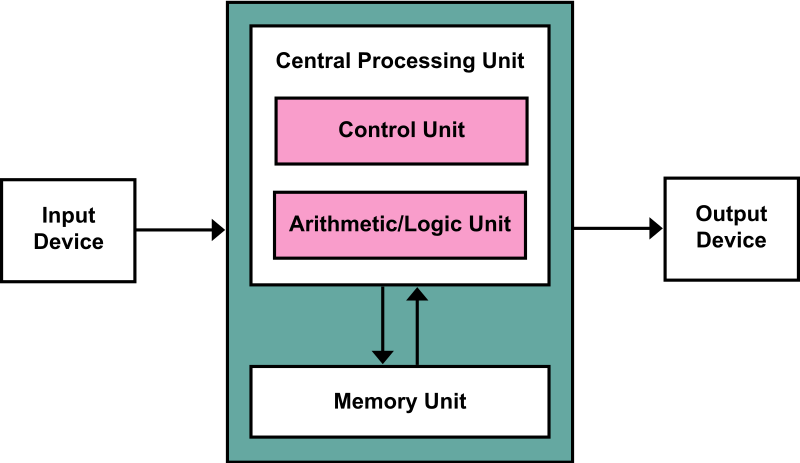
\includegraphics[width=\textwidth]{img/vonNeumannArchitecture.png}
\end{frame}

\begin{frame}
  \frametitle{Input/Output}
  \begin{block}{Input devices}
    \begin{itemize}
    \item Keyboard
    \item Mouse
    \end{itemize}
  \end{block}
  \pause
  \begin{block}{Output devices}
    \begin{itemize}
    \item Screen
    \item Printer
    \end{itemize}
  \end{block}
  \pause
  \begin{block}{Input/output devices}
    \begin{itemize}
    \item Hard disk
    \item Network card
    \end{itemize}
  \end{block}
\end{frame}

\begin{frame}
  \frametitle{Algorithms}
  \begin{itemize}
  \item a series of ordered \alert{steps}
  \item with the goal of performing a \alert{task}
  \end{itemize}
  \pause
  \begin{block}{Examples}
    \begin{itemize}
    \item a recipe
    \item an algebraic formula
    \end{itemize}
  \end{block}
\end{frame}

\begin{frame}
  \frametitle{Program}
  \begin{itemize}
  \item An implementation of an \alert{algorithm} in a certain
    \alert{programming language} (software)
    \pause
  \item A program can be \alert{executed} by a \alert{machine}
    (hardware)
    \pause
  \item Often a program need to be \alert{compiled} before the
    execution (\alert{transformed} in something understandable from the
    machine)
  \end{itemize}
\end{frame}

\begin{frame}
  \frametitle{Literary comparison}
  \begin{description}
  \item[Algorithm:] the history \\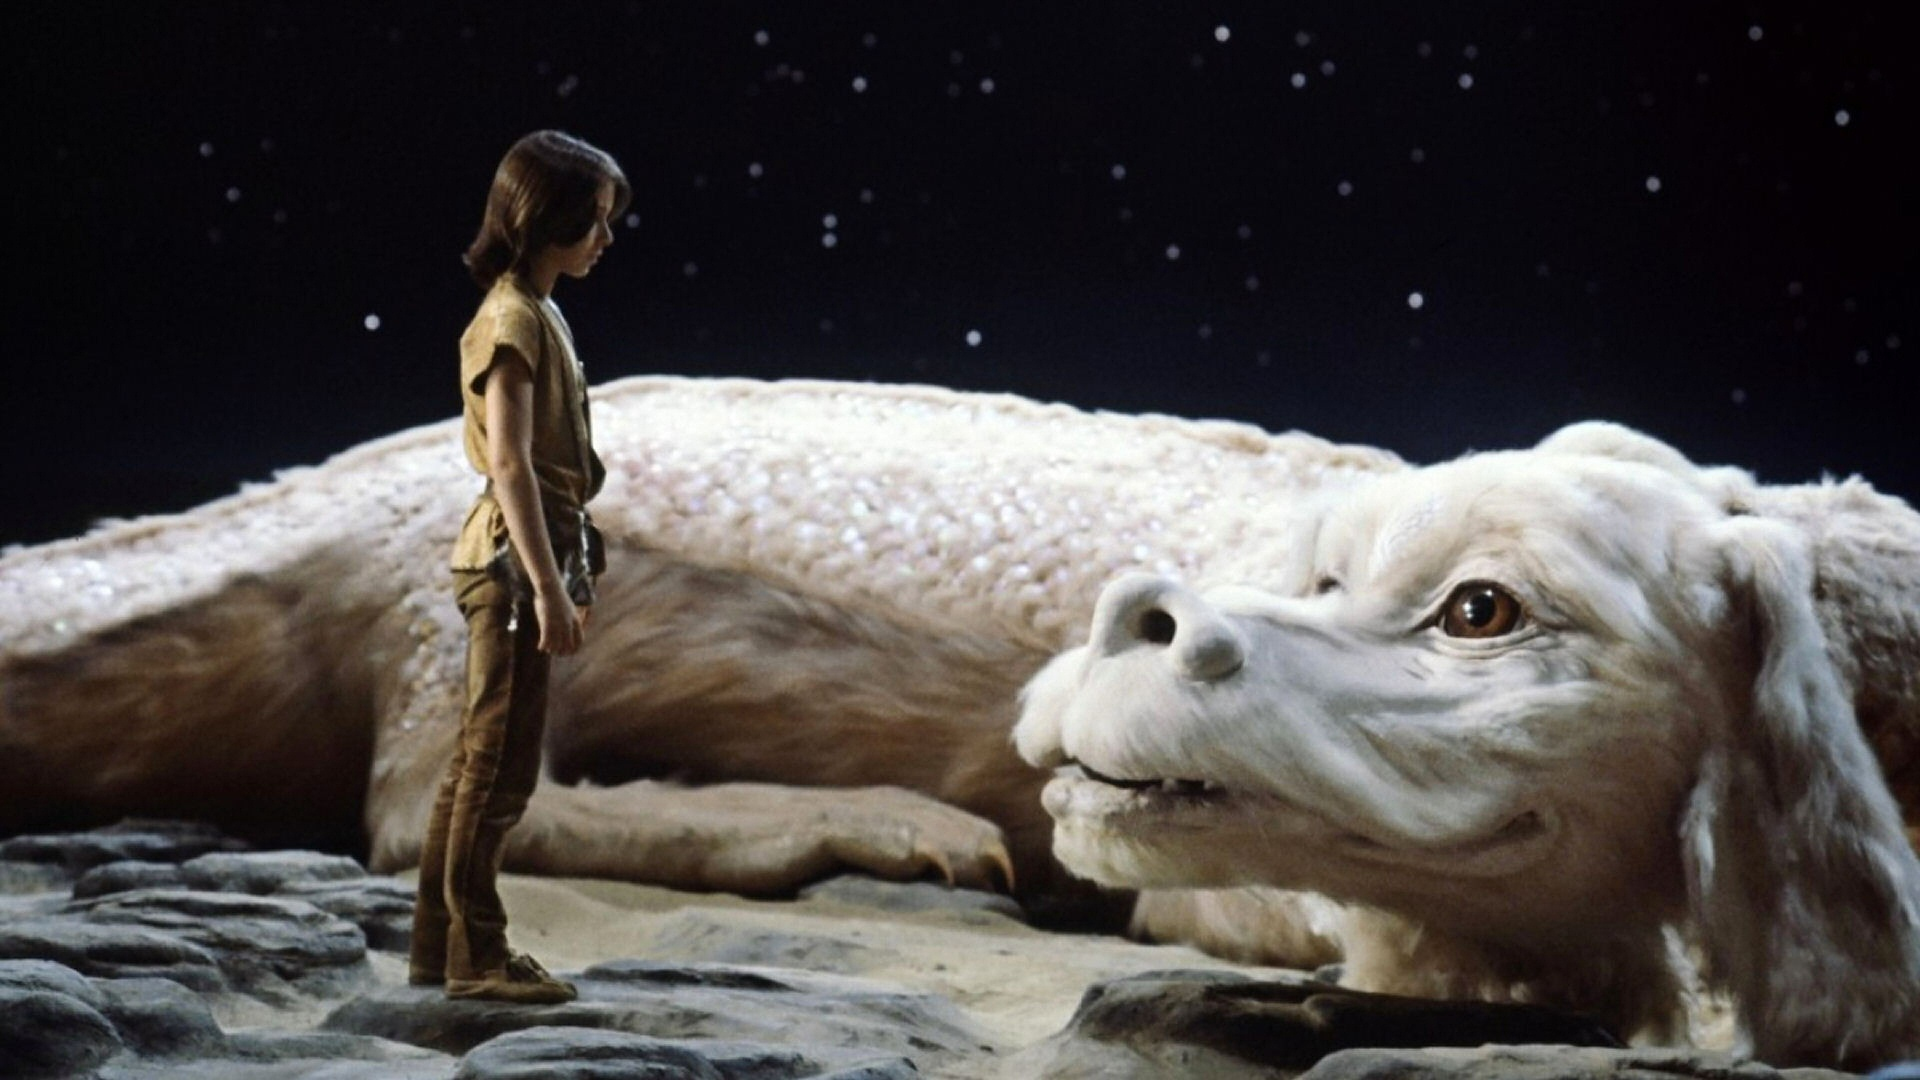
\includegraphics[width=3cm]{img/neverEndingStory1.jpeg}
  \item[Program:] the text\\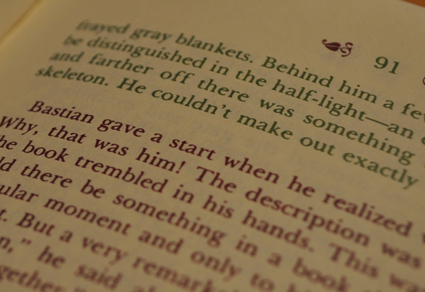
\includegraphics[width=3cm]{img/neverEndingStory2.jpeg}
  \item[Hardware:] the book\\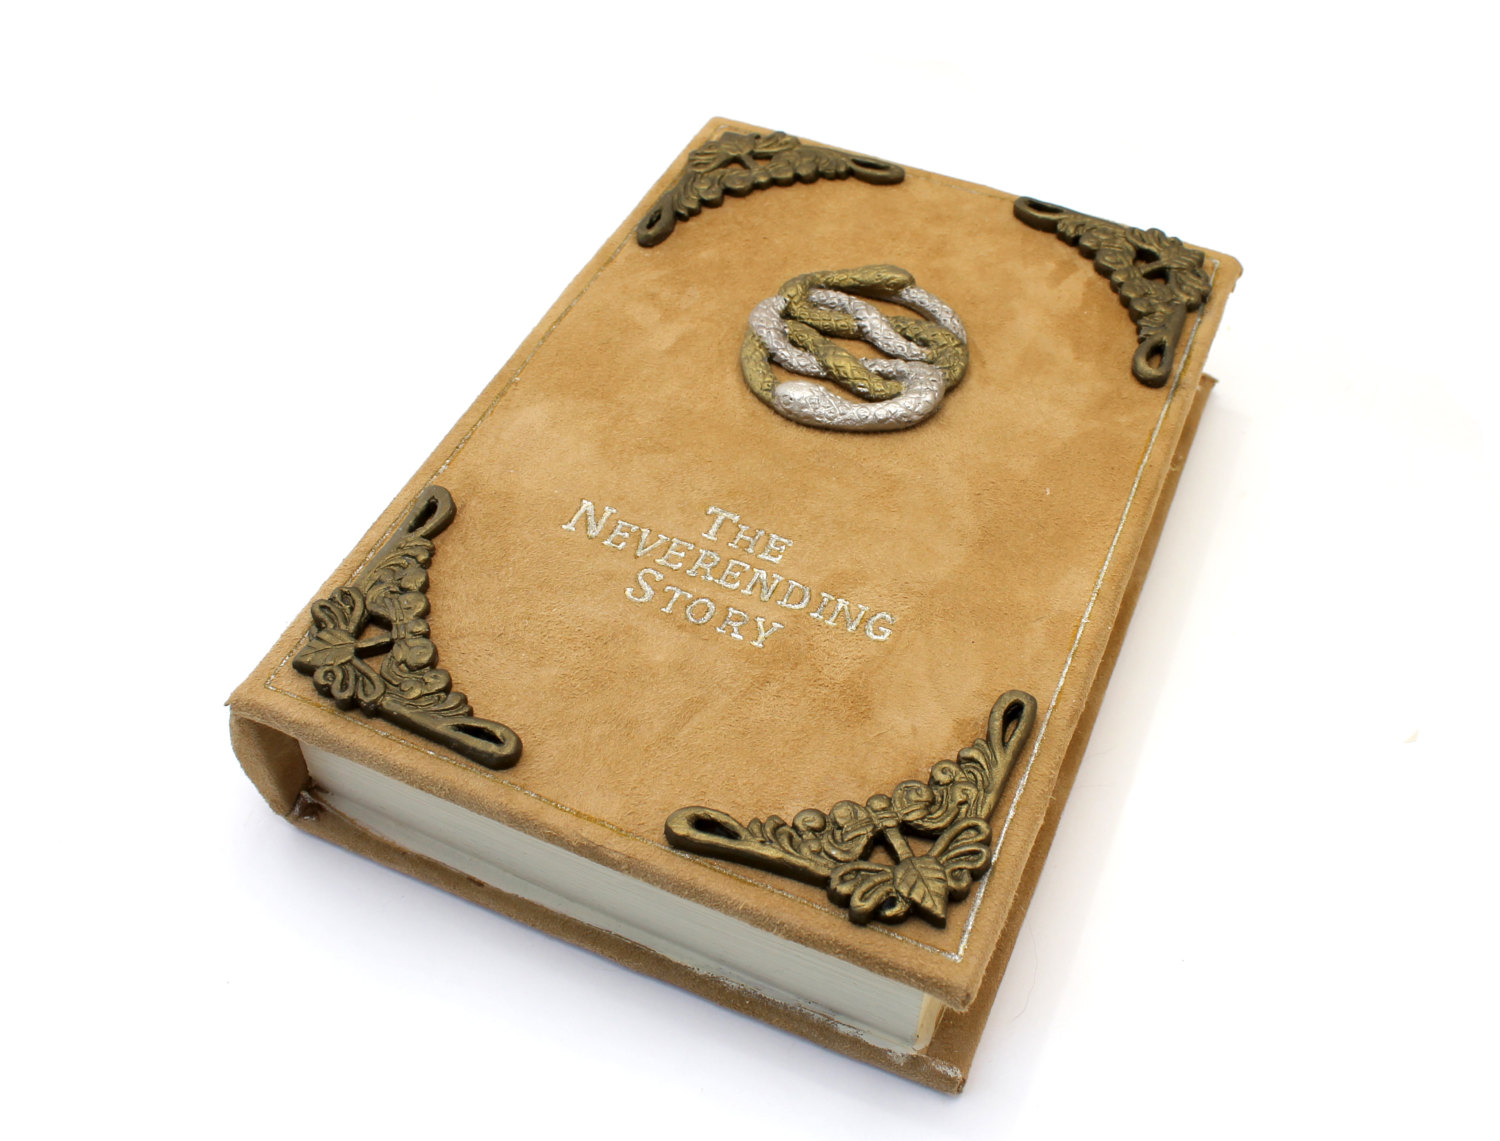
\includegraphics[width=3cm]{img/neverEndingStory3.jpeg}
  \end{description}
\end{frame}
\end{document}